\documentclass[a4paper, 12pt]{article}%тип документа

%отступы
\usepackage[left=2cm,right=2cm,top=2cm,bottom=3cm,bindingoffset=0cm]{geometry}

%Русский язык
\usepackage[T2A]{fontenc} %кодировка
\usepackage[utf8]{inputenc} %кодировка исходного кода
\usepackage[english,russian]{babel} %локализация и переносы

%Вставка картинок
\usepackage{wrapfig}
\usepackage{graphicx}
\graphicspath{{pictures/}}
\DeclareGraphicsExtensions{.pdf,.png,.jpg}

%оглавление
\usepackage{titlesec}
\titlespacing{\chapter}{0pt}{-30pt}{12pt}
\titlespacing{\section}{\parindent}{5mm}{5mm}
\titlespacing{\subsection}{\parindent}{5mm}{5mm}
\usepackage{setspace}

%Графики
\usepackage{multirow}
\usepackage{pgfplots}
\pgfplotsset{compat=1.9}

%Математика
\usepackage{amsmath, amsfonts, amssymb, amsthm, mathtools}

%Заголовок
\author{Балдин Виктор Алексеевич \\
группа Б01-303}
\date{}
\title{\textbf{Работа 4.3.1\\Дифракции Френеля и Фраунгофера}}
\newtheorem{task}{Задача}
\begin{document}
\maketitle
\textbf{Цель работы}: исследовать являения дифракции Френеля и Фраунгофера на щели, изучить влияние дифракции на разрешающую способность оптических инструментов.


\textbf{В работе используются}: оптическая скамья, ртутная лампа, монохроматор, щели с регулируемой шириной, рамка с вертикальной нитью, двойная щель, микроскоп на поперечных салазках с микрометрическим винтом, зрительная труба.
\section{Дифракция Френеля}
\subsection*{Установка}
\begin{figure}[h]
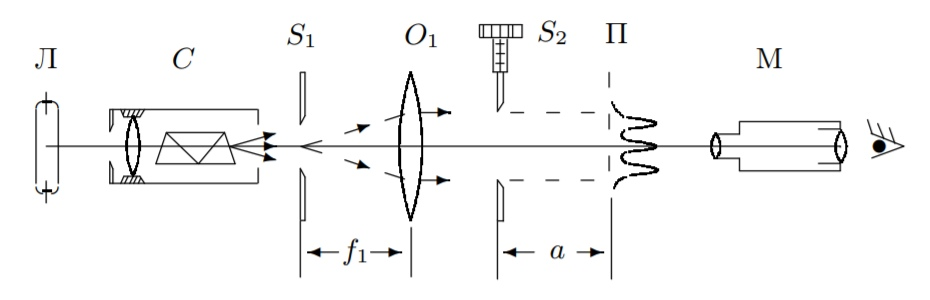
\includegraphics[width=0.7\textwidth]{7.jpg}
\centering
\caption{Схема установки.}
\end{figure}
Схема установки представлена на Рис. 1.\\
\subsection*{Теория}
Распределение интенсивности света в плоскости П рассчитаем с помощью зон Френеля. При освещении $S_2$ параллельным пучком лучей (плоская зона) зоны Френеля представляют собой плоскости, параллельные краям щели. Результирующая амплитуда в точке наблюдения определеяется суперпозицией колебаний от тех зон Френеля, которые не перекрыты створками щели. Графическое определение результирующей амплитуды производится с помощью векторной диаграммы -- спирали Корню. Суммарная ширина $m$ зон Френеля $z_m$ определяется соотношение
\begin{equation}
z_m = \sqrt{am\lambda},
\end{equation}
где $a$ -- расстояние от щели до плоскости П. Вид наблюдаемой картины определяется \textit{числом Френеля} $\Phi$:
$$
\Phi^2 = \dfrac{D}{\sqrt{a\lambda}}
$$
-- число зон Френеля, которые укладываются в ширине щели $D$. $p = \frac{1}{\Phi^2}$ называется \textit{волновым параметром}.
% \subsection*{Ход работы}
% \begin{enumerate}
% \item Соберем и настроим экспериментальную установку.
% \item Постепенно отодвигая микроскоп от $S_2$, отметим положение, при котором на фоне щели видна одна тёмная полоса. Смещение от начального положения даёт $a$.
% \item Измеряем ширину $D$ щели $S_2$ с помощью микрометрического винта и поперечных салазок микроскопа и
% \[D_{micro} = (2,855 \pm 0,005) \cdot 10^{-4} \text{м}\]
% \[D_{shel} = (2,75 \pm 0,05) \cdot 10^{-4} \text{м}\]
% В данных, написанных выше, берем погрешность, равную половине цены деления шкалы, то есть в случае микрометрического винта: $0,001/2$, а в случае салазок микроскопа: $0,01/2$.
% \item Проследим за изменением количества полос при изменении расстояния $a$. Принимая $x_0 = 46,8$ см, запишем все данные, которые мы получили, и из формулы $(1)$ получим $2z_m$, сравним из с $D$ и построим это все на графике. При расчетах используются $\lambda = 576,96$ нм.

% \begin{table}[h]
% \begin{center}
% \begin{tabular}{|c|c|c|c|c|c|}
% \hline
% количество полос m & $x$, см & $\delta x$, см & $a_m$, см & $2z_m$, мкм & $\delta(2z_m)$, мкм \\ \hline
% 1                  & 44,20    & 0,05           & 2,6       & 245         & 9                   \\ \hline
% 2                  & 45,00      & 0,05            & 1,8       & 289         & 16                  \\ \hline
% 3                  & 45,60    & 0,05            & 1,2       & 290         & 20                  \\ \hline
% 4                  & 465      & 0,05            & 0,8       & 270         & 30                  \\ \hline
% 5                  & 46,15    & 0,05           & 0,7       & 280         & 40                  \\ \hline
% 6                  & 46,25    & 0,05            & 0,6       & 290         & 40                  \\ \hline
% \end{tabular}
% \caption{Зависимость расстояния от щели до плоскости наблюдения от числа темных полос.}
% \end{center}
% \end{table}

% Погрешности в таблице выше получаются для $x$ из половины цены деления поперечных салазок микроскопа (было описано в пункте 3), а для $z_m$ из почленного дифференцирования формулы $(1)$, а именно погрешность для $z_m$ равна
% \[ \delta(2 z_m) = 2	z_m \cdot \sqrt{\left(\dfrac{\partial \left( 2\sqrt{a_mm\lambda} \right)}{\partial a_m}\right)^{2} \sigma_{a_m}^2} = 2 z_m \sqrt{\dfrac{m \lambda}{a_m}} \sigma_{a_m}\]
% А если вспомнить, что $z_m = \sqrt{a_m m \lambda}$, то формула погрешности примет вид, который использовался для подсчета погрешности в таблице:
% \[\delta(2z_m) = 2 m \lambda \sigma_{a_m}\]
% Усреднив $2z_m$ мы получим ширину щели $D$, погрешность для нее считается по формуле
% \[\delta D_{mid} = \dfrac{1}{\sqrt{n(n-1)}} \cdot \sqrt{\sum\limits_{i = 1}^n\left(D_i - D_{mid}\right)^2}\]
% и итоговая погрешность
% \[\delta D = D \cdot \sqrt{\sigma^2 (D)_{mid} + (\delta D/D)^2}\]
% Все это будет показано численно в выводе.
% \begin{figure}[h!]
% \begin{center}
% 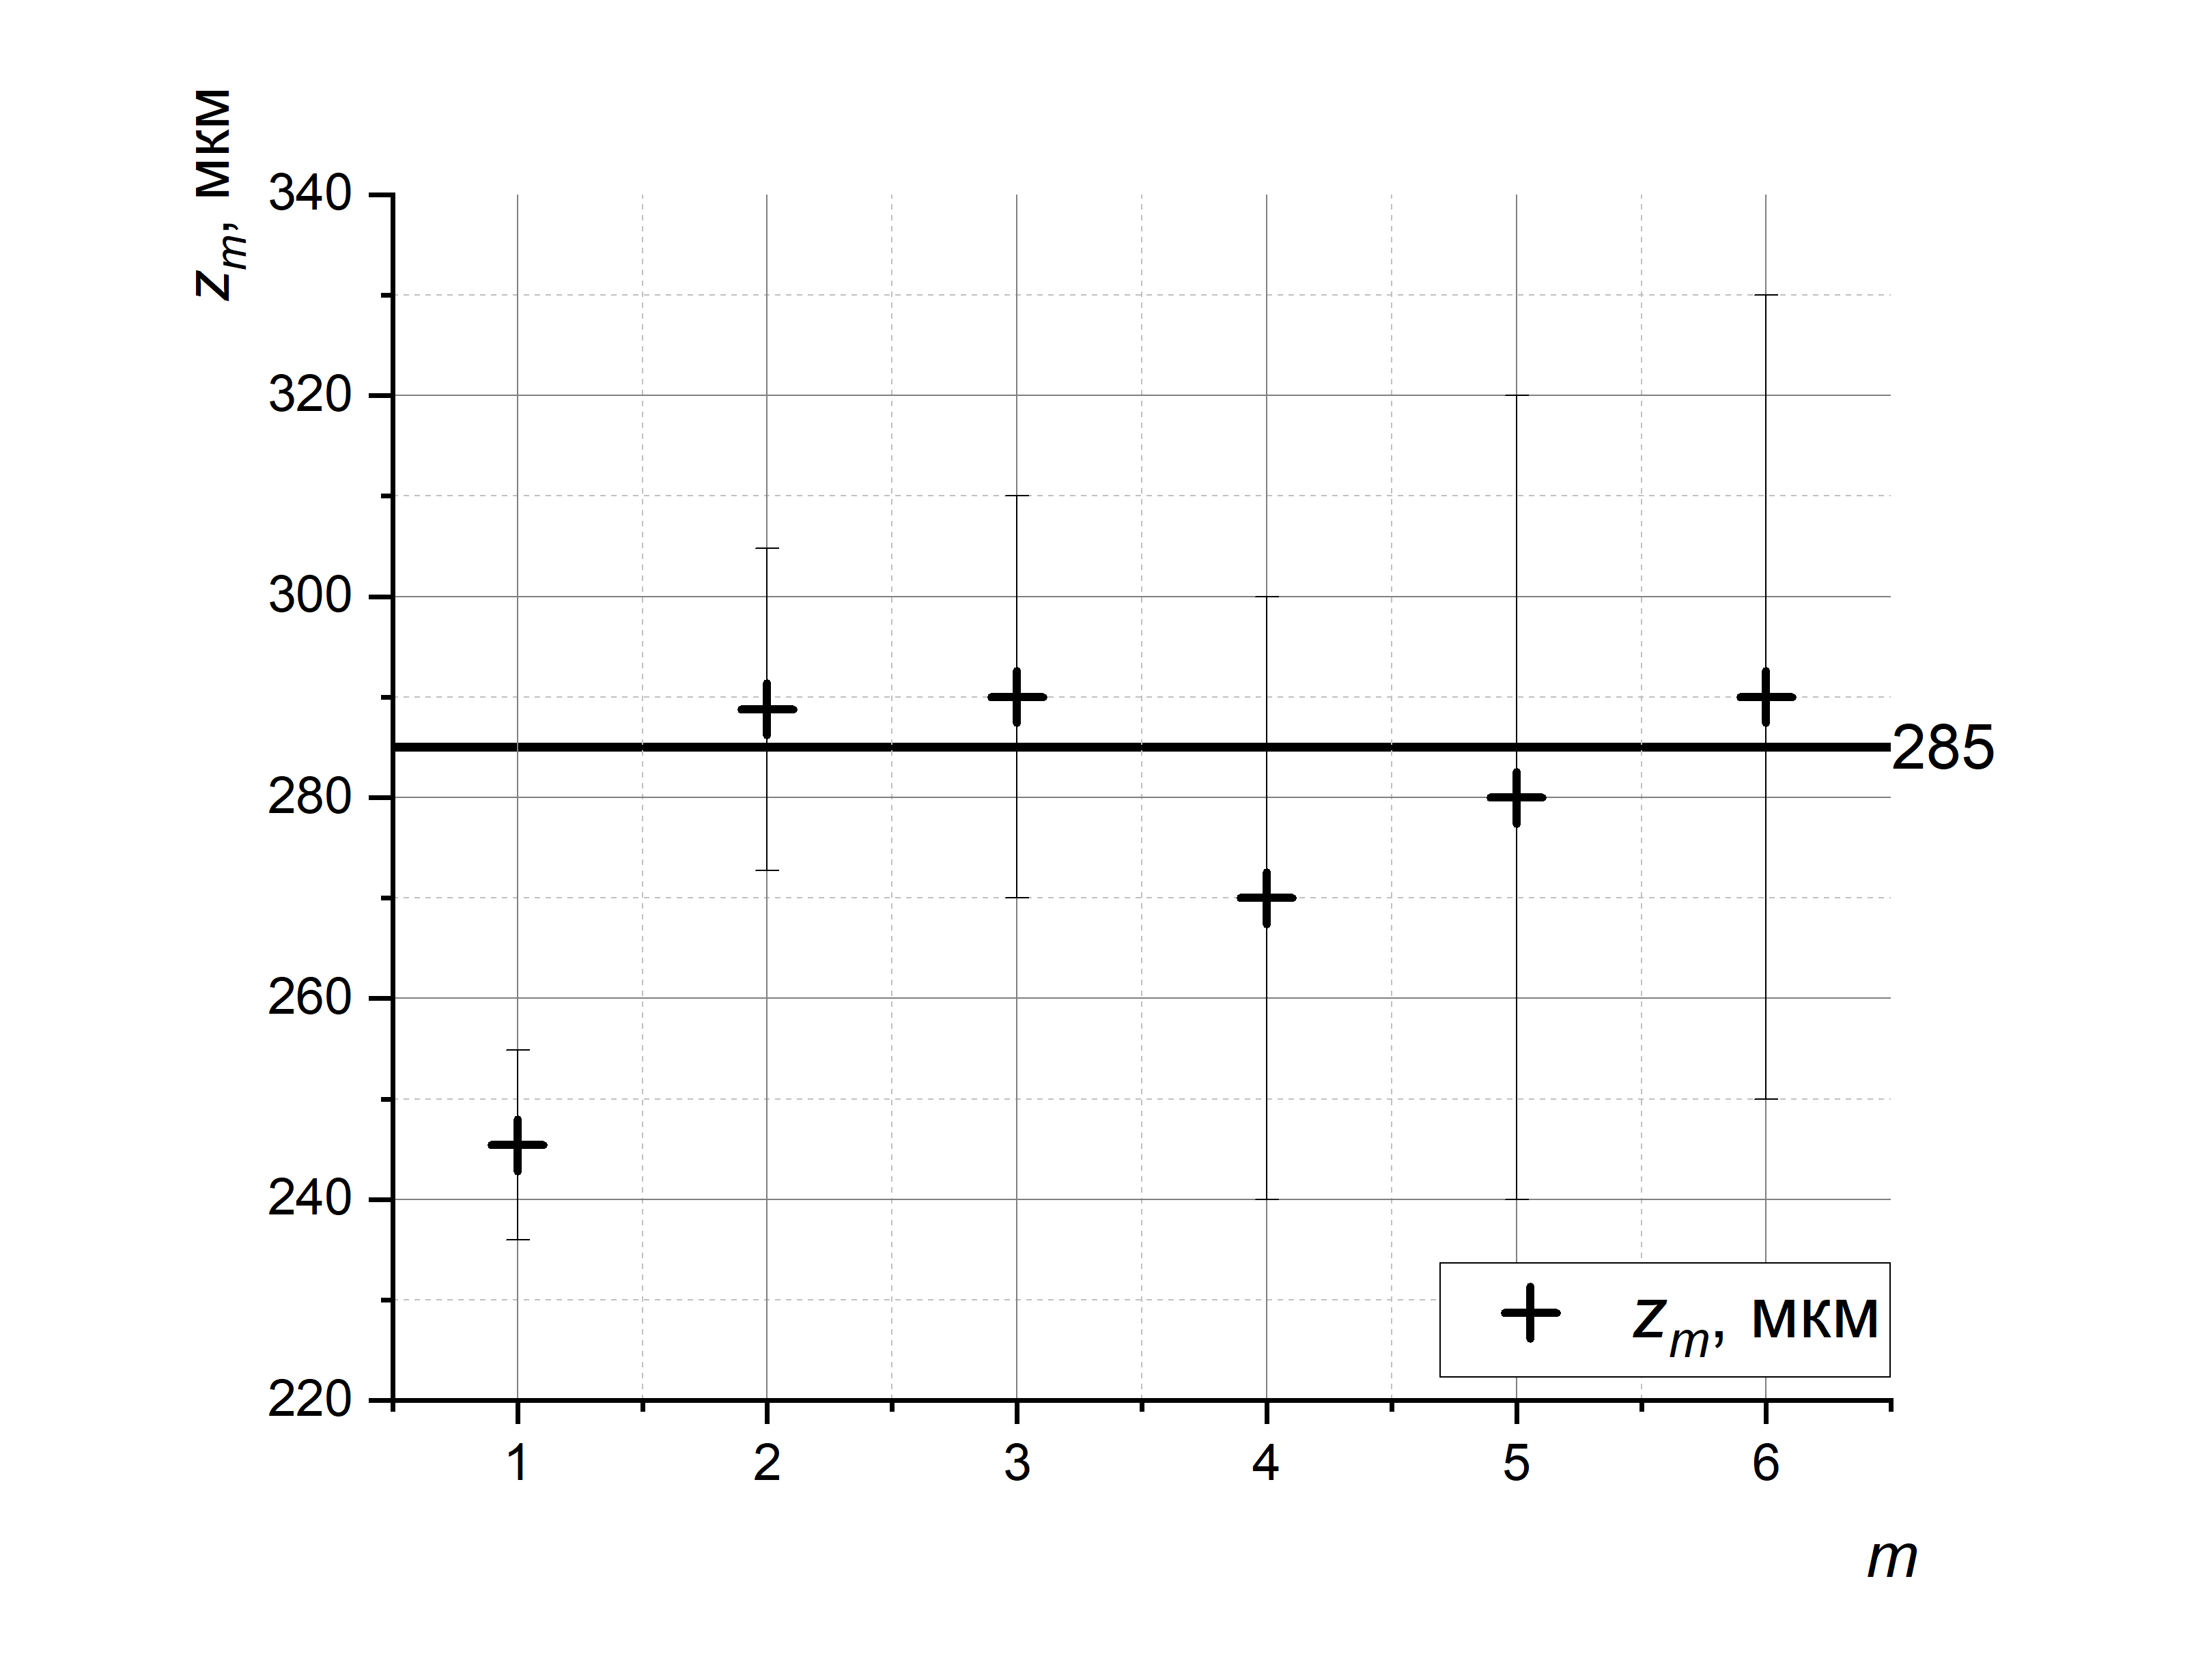
\includegraphics[width = 0.8\textwidth]{8.jpg}
% \caption{Визуализация данных, полученных в пункте А}
% \end{center}
% \end{figure}
% \end{enumerate}
\section{Дифракция Фраунгофера на щели}
\subsection*{Теория}
\begin{wrapfigure}{r}{0.5\textwidth}
  \begin{center}
    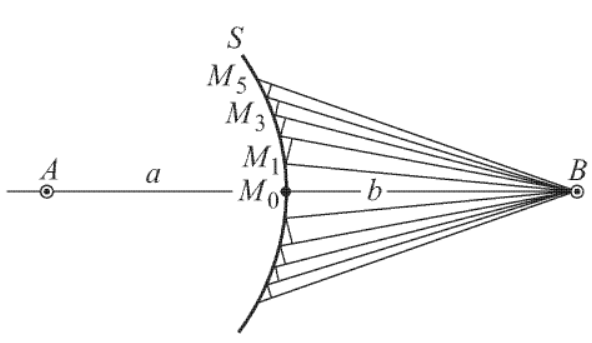
\includegraphics[width = 0.4\textwidth]{2.png}
  \end{center}
  \caption{Построение зон Френеля}
\end{wrapfigure}
Для выкладок ниже нам потребуется знать \textit{принцип Гюйгенса-Френеля}. Он формулируется следующим образом

\textit{Каждый элемент волнового фронта можно рассматривать как центр  вторичного возмущения, порождающего вторичные сферические волны, а результирующее световое поле  в каждой точке пространства будет определяться интерференцией этих волн.}

Теперь рассмотрим первое применение этого принципа, получившее название \textit{метод зон Френеля}

Для этого рассмотрим действие световой волны действующей из точки $A$ в какой-то точке $B$.

В этом случае можно, взяв точку $M_0$ в качестве центра (см. рис. 1), построить ряд концентрических сфер, радиусы которых начинаются с $b$ и увеличиваются каждый раз на половину длины волны $\lambda/2$. При пересечении с плоским фронтом волны $F$ эти сферы дадут концентрические окружности. Таким образом, на фронте волны появятся кольцевые зоны (зоны Френеля) с радиусами $r_1, r_2$ и т. д.

Из геометрических соображений посчитав, можно получить, что
\begin{equation}
r_i = i \sqrt{a \lambda}
\end{equation}
Введем так же обозначение: \textit{число Френеля}
\begin{equation}
\Phi^2 = \dfrac{D}{\sqrt{a\lambda}}
\end{equation}
\begin{wrapfigure}{r}{0.5\textwidth}
  \begin{center}
    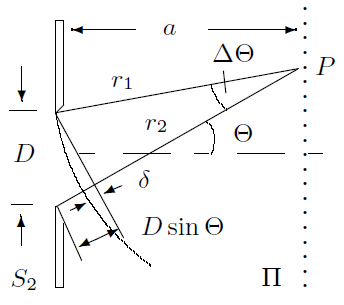
\includegraphics[width = 0.35\textwidth]{1.png}
  \end{center}
  \caption{К фазовым соотношениям при дифракции Фраунгофера}
\end{wrapfigure}
В этом пункте рассмотрим дифракцию, когда ширина щели становится значительно меньше ширины первой зоны Френеля, т.е. если
\begin{equation}
D \ll\sqrt{a \lambda}
\end{equation}
Это условие всегда выполняется при достаточно большом $a$. В этом случае говорят, что \textit{дифракция Фраунгофера}. При выполнении пункта $(2)$ у нас заметно упрощаются фазовые соотношения, что поясняет рис. 2, в итоге с хорошим приближением можно считать, что разность хода между соседними лучами равна
\begin{equation}
\Delta = r_2 - r_1 \approx D \sin \theta \approx D \cdot \theta
\end{equation}
Здесь предполагается, что $\theta$ достаточно мал.

\subsection*{Схема установки}
Дифракцию Фраунгофера можно наблюдать на подобной установке

\begin{figure}[h]
\begin{center}
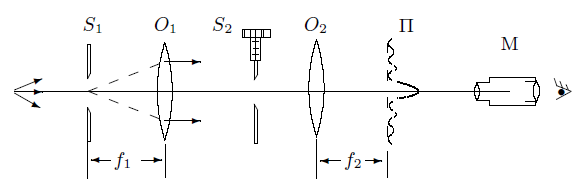
\includegraphics[width = 0.7\textwidth]{3.png}
\caption{Схема установки для пункта 2}
\end{center}
\end{figure}

Объектив здесь нужен для удобства, так как неудобно работать с очень узкими щелями. Дифракционная картина здесь наблюдается в фокальной плоскости объектива $O_2$.

Посчитав легко определить угловую координату любой темной полосы:
\begin{equation}
\theta_m = \frac{m \lambda}{D}
\end{equation}
И расстояние от центра соответственно
\begin{equation}
X_m = f_2m\frac{\lambda}{D}
\end{equation}
\section*{Ход работы}
\subsection*{Дифракция Френеля}
\subsubsection*{1-4}
Соберем установку на рис. 1. Для этого включим ртутную лампу и поставим после нее фильтр с щелью. После щели нужно будет поставить линзу так, чтобы щель была в фокусе. Для этого воспользуемся зрительной трубой, настроенной на бесконечность. Поскольку, если линза находится в нужном месте, из нее выходит пучок параллельных лучей, зрительная труба, настроенная на бесконечность, должна показать четкое изображение щели. После установки линзы поместим щель $S_2$ и микроскоп после неё. На этом сборка установки завершена.
\subsubsection*{5}
Найдем нуль микрометрического винта щели $S_2$. Для этого посмотрим свозь щель на лампу накаливания и начнем поворачивать винт из нулевого положения до тех пор, пока свет от лампы не станет виден. При этом положение винта будет нулем.

\begin{center}
\begin{tabular}{|c|c|c|c|}
\hline
$d, \text{мкм}$&$20$&$17$&$18$\\ \hline
\end{tabular}\\~\\
$\Delta d = 0.5, \text{мкм}$
\end{center}
\[<d> = 18.3 \pm 1.0, \text{мкм}\]

(Погрешность $d$ была посчитана как корень суммы квадратов статистической и приборной).

\subsubsection*{6-9}

Поставив микроскоп за щелью, получим дифракционную картину. Заметим, что количество полос должно увеличиваться по мере отодвигания микроскопа от щели.

\begin{center}
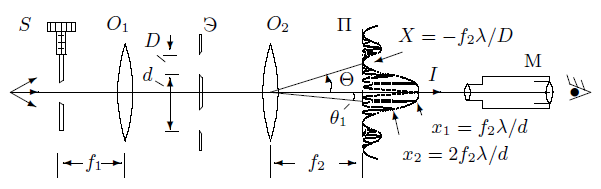
\includegraphics[width=0.80\textwidth]{4.png}
\end{center}

Измерим положение микроскопа $x$, при котором видно $n$ полос и найдем расстояние $a$ доплоскостии наблюдения, которое равно смещению относительно положения $x_0=540.0\pm0.5\,\text{мм}$

\begin{center}
\begin{tabular}{|c|c|c|c|c|c|c|}\hline
$n$&$x_{min}\text{, \text{мм}}$&$x_{max}\text{, \text{мм}}$&$x\text{, \text{мм}}$&$\Delta x\text{, \text{мм}}$&$a\text{, \text{мм}}$&$\Delta a\text{, \text{мм}}$\\\hline
$1.0$&$525.0$&$532.0$&$529$&$4$&$12$&$4$\\\hline
$2.0$&$532.0$&$535.0$&$533.5$&$1.6$&$6.5$&$1.7$\\\hline
$3.0$&$535.0$&$536.0$&$535.5$&$0.7$&$4.5$&$0.9$\\\hline
$4.0$&$536.0$&$536.0$&$536.0$&$0.5$&$4.0$&$0.7$\\\hline
$5.0$&$536.0$&$537.0$&$536.5$&$0.7$&$3.5$&$0.9$\\\hline
\end{tabular}\\~\\
$\Delta n=0\,\text{}, \Delta x_{min}=0.5\,\text{\text{мм}}, \Delta x_{max}=0.5\,\text{\text{мм}}$
\end{center}



Поскольку суммарная ширина зон френеля не меняется и равна $D$, из формулы $(1)$ следует, что зависимость между $a$ и $1/m$ должна быть линейной, что и видно из следующего графика

\begin{center}
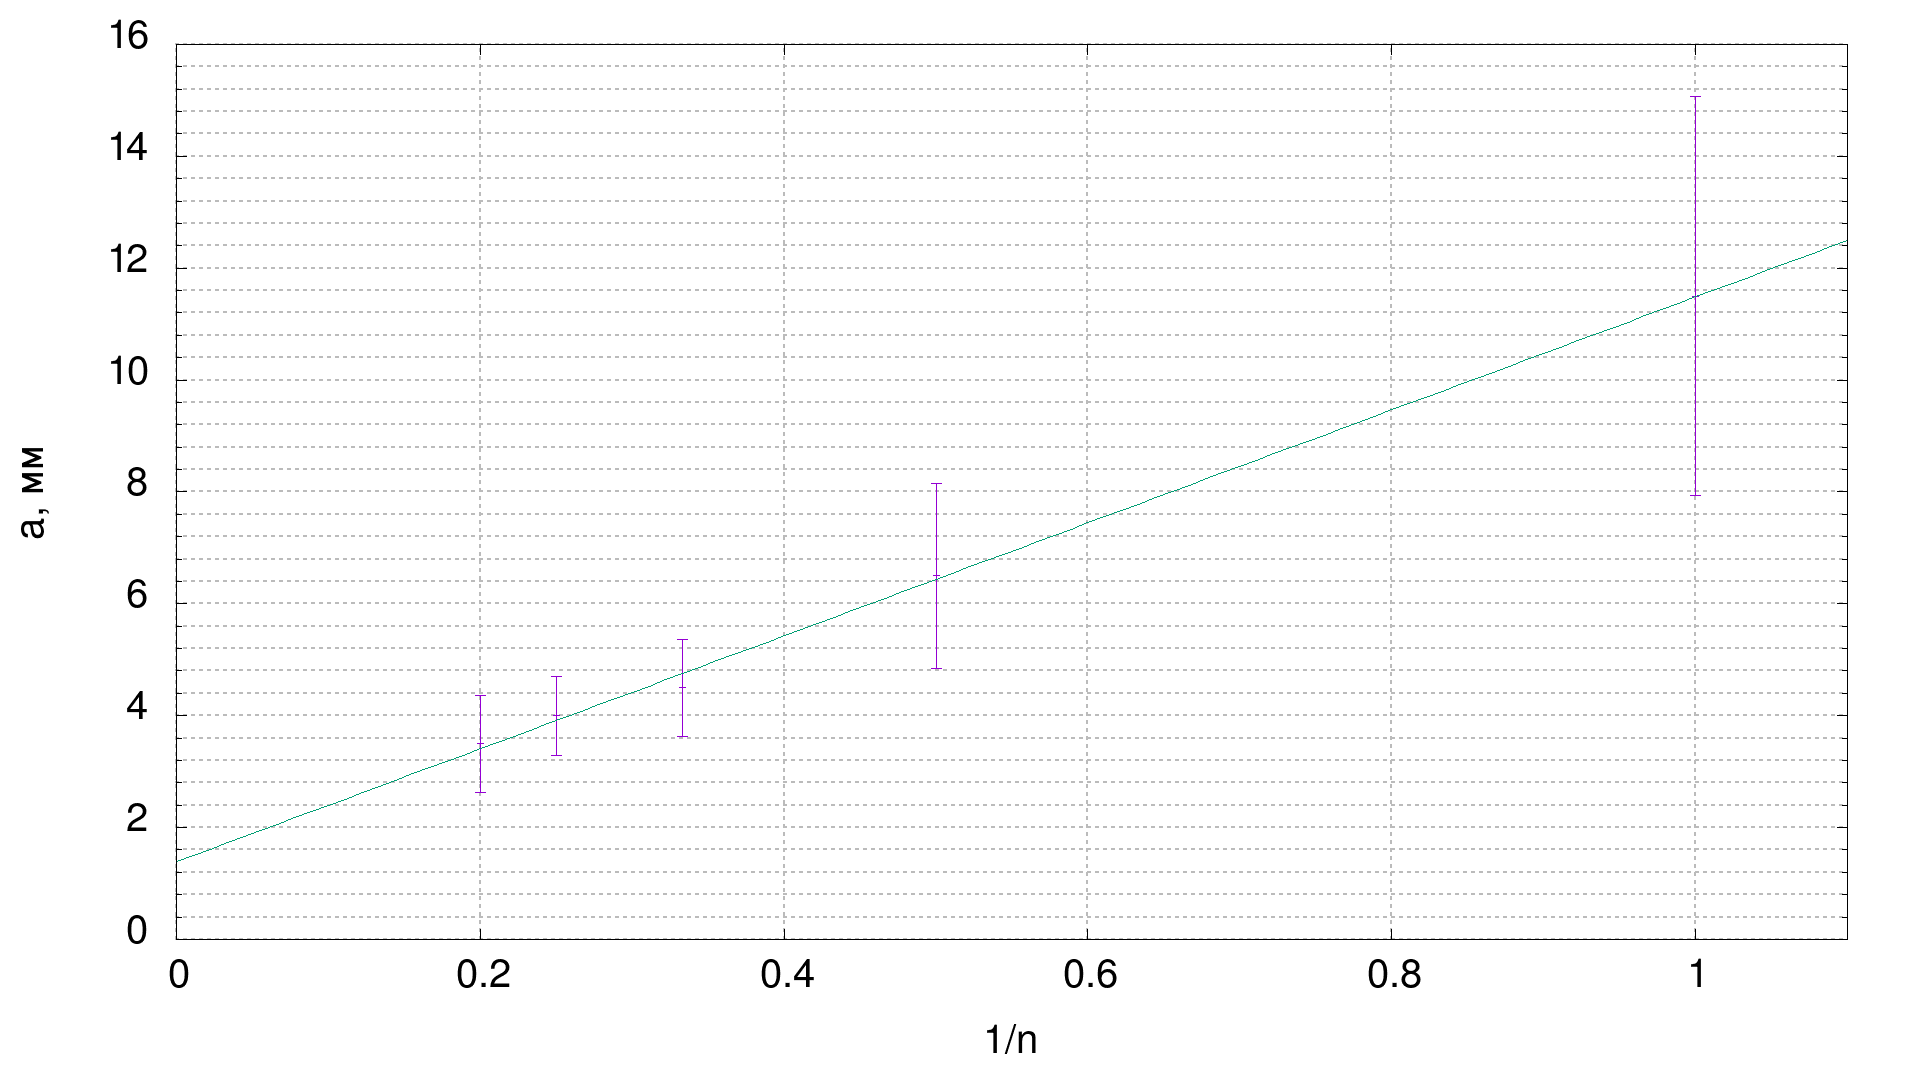
\includegraphics[width=0.80\textwidth]{plot1.png}.
\end{center}

Заметим, что вертикальный сдвиг линейной зависимости равен $1.3\,\text{мм}$ и находится в пределах погрешности.\\

\subsubsection*{10-11}

Независимо змерим ширину щели с помощью микроскопа и микрометра.

\begin{center}
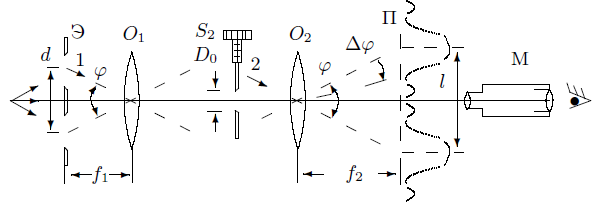
\includegraphics[width=0.80\textwidth]{5.png}\\
Иллюстрация, не является измерением.
\end{center}

В результате получилось

\[d_{\text{мех}}=(258-18)\pm1.1\,\text{мкм}=240\pm1.1\,\text{мкм}\]
\[d_{\text{опт}}=240\pm10\,\text{мкм}\]

\subsubsection*{12}

Для исследования дифракции Френеля на препятствии, поставим в место щели $S_2$ тонкую вертикальную нить и настроим микроскоп на ее резкое изображение

\begin{center}
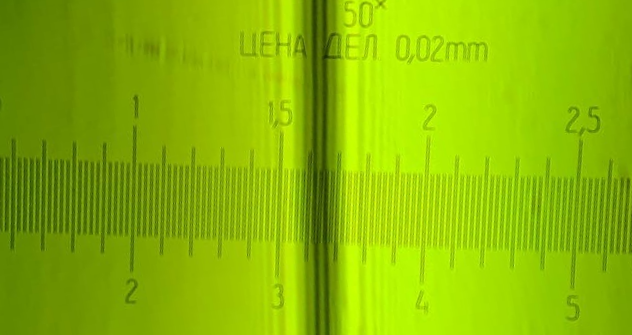
\includegraphics[width=0.80\textwidth]{6.png}.\\
\end{center}

При удалении от нити всегда наблюдается четное число темных дифракционных полос.

\subsection{Дифракция Фраунгофера на щели}

\subsubsection*{1-3}
Для того, чтобы наблюдать дифракцию френеля, нужно поставить еще одну линзу $O_2$ после щели, чтобы в ее фокальной плоскости появилась картина из параллельных лучей. После этого достаточно настроить микроскоп на эту фокальную плоскость, сняв щель $S_2$ со скамьи и получив четкое изображение щели $S_1$ в окуляре.
\subsubsection*{4-7}
Пронаблюдаем дифракционную картину
\begin{center}
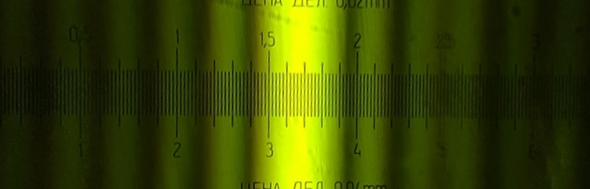
\includegraphics[width=0.80\textwidth]{7.png}.\\
\end{center}

\begin{center}
\begin{tabular}{|c|c|c|c|}\hline
$m$&$x_{min}\text{, \text{мм}}$&$x_{max}\text{, \text{мм}}$&$x\text{, \text{мм}}$\\\hline
$-5.0$&$0.26$&$0.38$&$0.320$\\\hline
$-4.0$&$0.54$&$0.64$&$0.590$\\\hline
$-3.0$&$0.80$&$0.90$&$0.850$\\\hline
$-2.0$&$1.08$&$1.18$&$1.130$\\\hline
$-1.0$&$1.36$&$1.42$&$1.390$\\\hline
$1.0$&$1.94$&$1.98$&$1.960$\\\hline
$2.0$&$2.16$&$2.28$&$2.220$\\\hline
$3.0$&$2.48$&$2.52$&$2.500$\\\hline
$4.0$&$2.72$&$2.86$&$2.790$\\\hline
$5.0$&$3.00$&$3.10$&$3.050$\\\hline
\end{tabular}\\~\\
$\Delta m=0\,\text{}, \Delta x_{min}=0.01\,\text{\text{мм}}, \Delta x_{max}=0.01\,\text{\text{мм}}, \Delta x=0.014\,\text{\text{мм}}$
\end{center}



\begin{center}
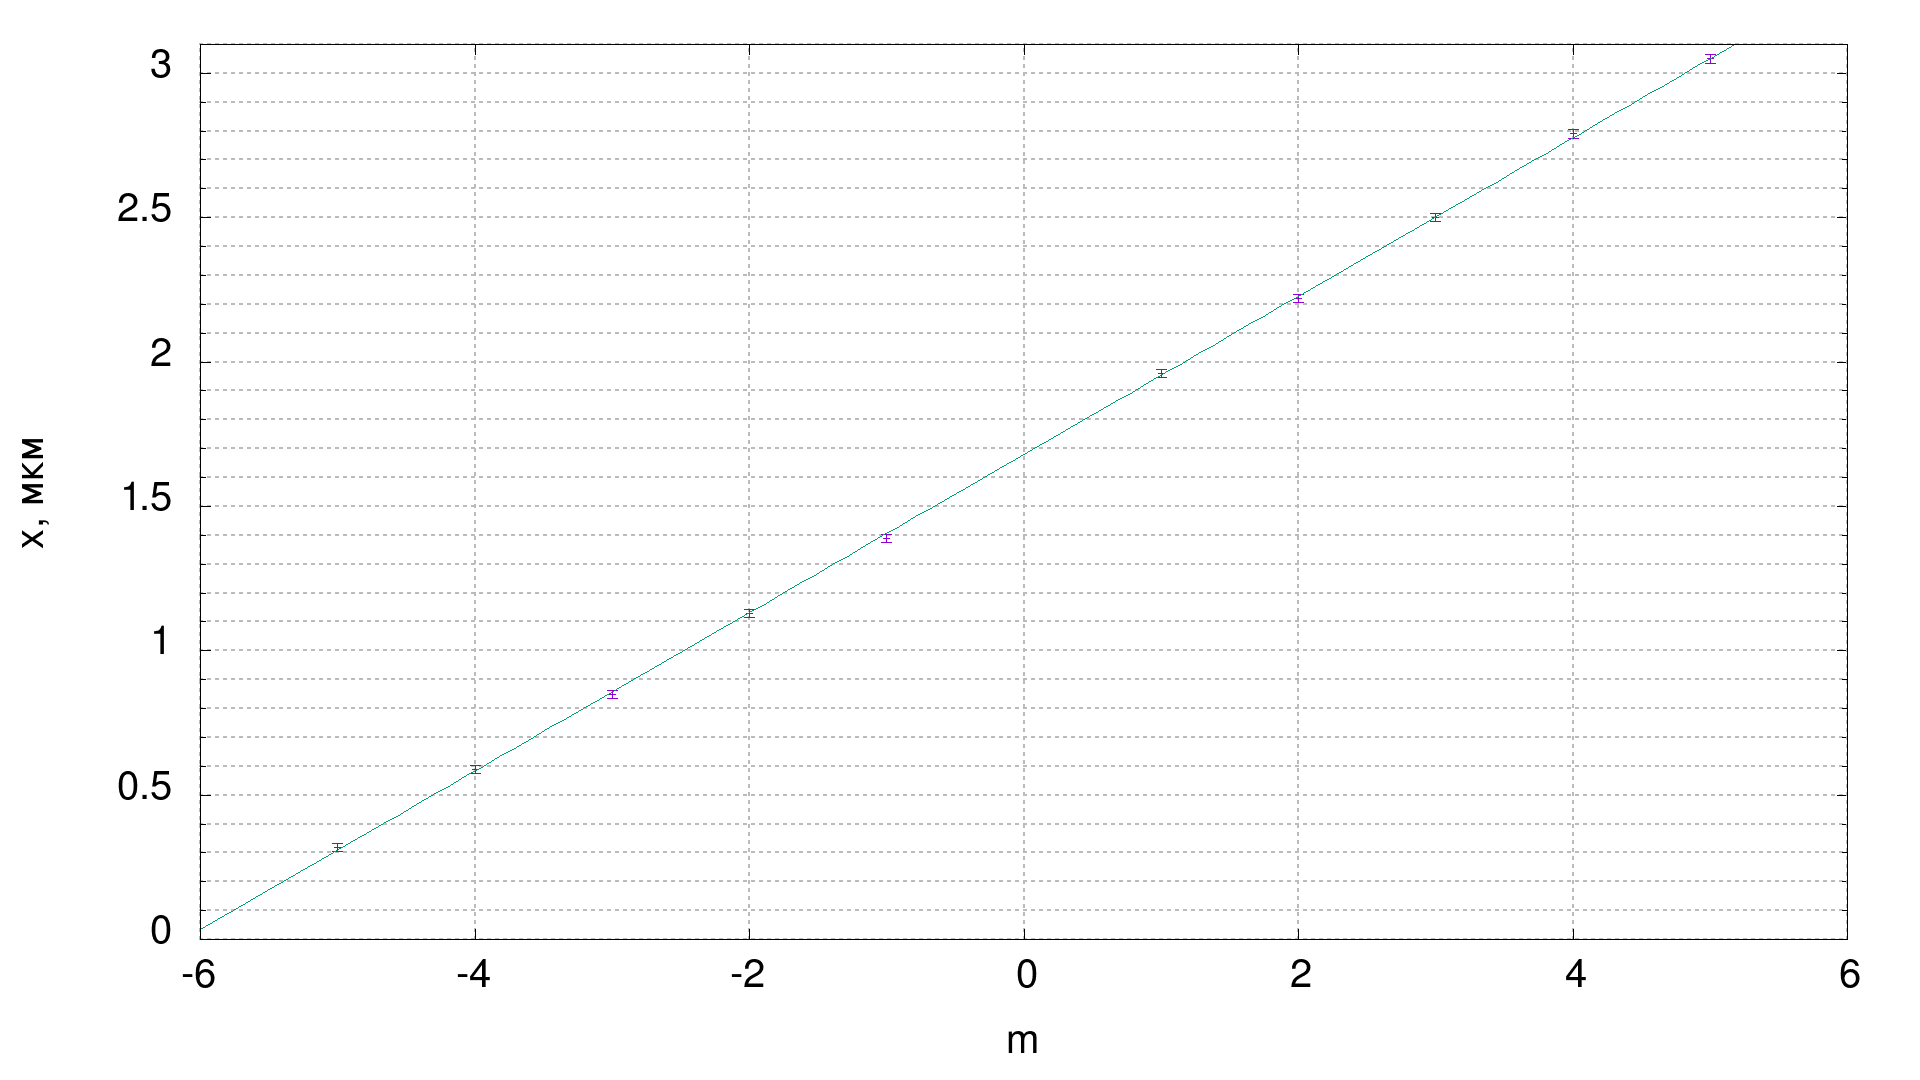
\includegraphics[width=0.80\textwidth]{8.png}.\\
\end{center}

Измерение проводились при ширине щели

\[D=(17.0\pm0.5)\times20\,\text{мкм}=340\pm10\,\text{мкм}.\]

И фокусном расстоянии линзы

\[f=160\,\text{мм}\]

Если $A = (274.0\pm0.9)\,\text{мкм}$ -- угол наклона графика, то
\[\lambda = D \frac{A}{f} = 582\pm19\,\text{нм}\]

\section*{Вывод}

Мы изучили два основных типа дифракции: Френеля и Фраунгофера при разных размерах щели и провели качественные наблюдения этих явлений, а также экспериментально проверили справедливость теоретических формул.

\end{document}

\end{document}